\documentclass{article}
\begin{document}
\subsection{GPIO mapping}

\subsubsection{GPIO mapping of APP2.0 shuttle board pins}

The APP2.0 shuttle board has total of 28 pins, of which some have a predefined functionality and some can be used as GPIO by the user.

The shuttle board connector details are given in the table below.

\begin{table}[H]
	\centering
	\begin{tabular}{|c|c|c|c|}
		\hline
		\textbf{Pin number on} & \textbf{Name /} & \textbf{Pin number on} & \textbf{Name /} \\
		\textbf{shuttle board} & \textbf{function} & \textbf{shuttle board} & \textbf{function} \\
		\hline\hline
		1 & VDD (3.3V) & 28 & SHTLE\_COD \#4 \\ \hline
		2 & VDDIO (3.3V) & 27 & SHTLE\_COD \#3 \\ \hline
		3 & GND & 26 & SHTLE\_COD \#2 \\ \hline
		4 & SPI MISO & 25 & SHTLE\_COD \#1 \\ \hline
		5 & SPI: MOSI / I\textsuperscript{2}C: SDA & 24 & SHTLE\_COD \#0 \\ \hline
		6 & SPI: SCK / I\textsuperscript{2}C: SCL & 23 & SHTLE\_COD\_GND \\ \hline
		7 & SPI: CS & 22 & IO\_4 ( GPIO \#4 ) \\ \hline
		8 & IO\_5 ( GPIO \#5 ) & 21 & IO\_7 ( GPIO \#7 ) \\ \hline
		9 & IO\_0 ( GPIO \#0 ) & 20 & IO\_6 ( GPIO \#6 ) \\ \hline 
		10 & SHTLE\_COD \#5 & 19 & IO\_8 ( GPIO \#8 ) \\ \hline 
		11 & SHTLE\_COD \#6 & 18 & SCL (see note) \\ \hline 
		12 & SHTLE\_COD \#7 & 17 & SDA (see note)\\ \hline 
		13 & SHTLE\_COD \#8 & 16 & IO\_3 ( GPIO \#3 ) \\ \hline
		14 & IO\_1 ( GPIO \#1 ) & 15 & IO\_2 ( GPIO \#2 ) \\ \hline
	\end{tabular}
	\caption{Overview of shuttle board pins and their function}
	\label{tab:shtbrdpins}
\end{table}

Note:
\begin{itemize}
	\item In COINES functions, the pins are addressed using the same numbers as on the shuttle board. For example, the GPIO \#5 has the pin number 8.
	\item In some cases (depending on the sensor), the I\textsuperscript{2}C lines are shuttle board pin 6 for the clock signal SCL and shuttle board pin 5 for the data line SDA. In such cases pins 17 and 18 may not be connected. Please carefully read the shuttle board documentation.
\end{itemize}

\subsubsection{GPIO mapping of APP3.x shuttle board pins}

The APP3.x shuttle board has a total of 16 pins, 7 on the left and 9 on the right. (with shuttle board pins facing downwards)

Note:
\begin{itemize}
	\item In COINES functions, the pins are addressed as on the APP3.x shuttle board. For example, the GPIO \#5 is addressed as \texttt{COINES\_MINI\_SHUTTLE\_PIN\_2\_6}.
	\item Supported VDD voltages on APP3.x are 0, 1.8V and 2.8V.
	\item Supported VDDIO voltage on APP3.x is 1.8V.
\end{itemize}

\begin{table}[H]
	\centering
	\begin{tabular}{|c|c|c|c|}
		\hline
		\textbf{Pin number on} & \textbf{Name /} & \textbf{Pin number on} & \textbf{Name /} \\
		\textbf{shuttle board} & \textbf{function} & \textbf{shuttle board} & \textbf{function} \\
		\hline\hline
		1\_1 & VDD (1.8/2.8V) & 2\_1 & SPI\_CS \\ \hline
		1\_2 & VDDIO (1.8) & 2\_2 & SPI: SCK / I\textsuperscript{2}C: SCL \\ \hline
		1\_3 & GND & 2\_3 & SPI: MISO \\ \hline
		1\_4 & GPIO0 & 2\_4 & SPI: MOSI /  I\textsuperscript{2}C: SDA \\ \hline
		1\_5 & GPIO1 & 2\_5 & GPIO4\textsuperscript{*} \\ \hline
		1\_6 & GPIO2 & 2\_6 & GPIO5\textsuperscript{*} \\ \hline
		1\_7 & GPIO3 & 2\_7 & IOXP\_INT\textsuperscript{*}\\ \hline
		     &       & 2\_8 & PlugDet\textsuperscript{*} \\ \hline
		     &       & 2\_9 & EEPROM\_RW \\ \hline
	\end{tabular}
	\caption{Overview of APP3.x shuttle board pins and their function}
	\label{tab:shtbrdpins}
	\textsuperscript{*}SPI pins for secondary interface - CS:GPIO4, SCK:GPIO5, MISO:IOXP\_INT, MOSI:PlugDet
\end{table}

\newpage
\subsection{COINES C functions}\label{CoinesCFunctions}
\subsubsection{coinesAPI calls: Interface and board information}

\paragraph{coines\_open\_comm\_intf}
Opens the communication interface.

\begin{lstlisting}
int16_t coines_open_comm_intf(enum coines_comm_intf intf_type,void *arg); 
\end{lstlisting}

In case of MCU Target, API waits indefinitely for serial port or BLE connection (\texttt{MCU\_APP30} target and \texttt{MCU\_APP31} target).

In case of PC Target, one can configure communication settings either by passing the address of \texttt{coines\_serial\_com\_config} or \texttt{ble\_peripheral\_info} to \texttt{*arg}.

Serial\ com\ configuration:
\newline If \texttt{*arg} is NULL for \texttt{COINES\_COMM\_INTF\_USB}, first com port enumerated will be used for communication.
The serial com configuration structure contains the following items. Refer to \ref{serialComConfig} for its implementation.

\begin{lstlisting}
struct coines_serial_com_config
{
	uint32_t baud_rate; /*< Baud rate */
	uint16_t vendor_id; /*< vendor Id */
	uint16_t product_id; /*< Product Id */
	char* com_port_name; /*< serial com port name */
	uint16_t rx_buffer_size; /*< RX response buffer size */
};
\end{lstlisting}

BLE\ com\ configuration:
\newline If \texttt{*arg} is NULL for \texttt{COINES\_COMM\_INTF\_BLE}, the nearest Application board for the host BLE will be used for communication.
The ble com configuration structure contains the following items. Refer to \ref{bleComConfig} for its implementation.

\begin{lstlisting}
struct ble_peripheral_info
{
	char ble_address[COINES_CHAR_MAX_LEN]; /*< BLE device address */
	char ble_identifier[COINES_CHAR_MAX_LEN]; /*< BLE device identifier */
};
\end{lstlisting}

\paragraph{coines\_close\_comm\_intf}
Closes the communication interface.

\begin{lstlisting}
int16_t coines_close_comm_intf(enum coines_comm_intf intf_type,void *arg); 
\end{lstlisting}

\paragraph{coines\_get\_board\_info}
Gets the board information.

\begin{lstlisting}
int16_t coines_get_board_info(struct coines_board_info *data);
\end{lstlisting}

The data structure contains the following items 

\begin{lstlisting}
struct coines_board_info {
	/*!Board hardware ID */
	uint16_t hardware_id;
	/*!Board software ID */
	uint16_t software_id;
	/*!Type of the board like APP2.0, Arduino Due*/
	uint8_t board;
	/*!Shuttle ID of the sensor connected*/
	uint16_t shuttle_id;
};
\end{lstlisting}

\subsubsection{coinesAPI calls: GPIO oriented calls}

\paragraph{coines\_set\_pin\_config}
Sets the pin direction and the state.

\begin{lstlisting}
int16_t coines_set_pin_config(enum coines_multi_io_pin pin_number, enum coines_pin_direction direction, enum coines_pin_value pin_value);  
\end{lstlisting}

\paragraph{coines\_get\_pin\_config}
Gets the pin configuration.

\begin{lstlisting}
int16_t coines_get_pin_config(enum coines_multi_io_pin pin_number, enum coines_pin_direction *pin_direction, enum coines_pin_value *pin_value);
\end{lstlisting}

\paragraph{coines\_set\_shuttleboard\_vdd\_vddio\_config}
Configures the VDD and VDDIO of the sensor. For APP2.0, a voltage level of 0 or 3300 mV is supported. Any values above 0 will default to 3300 mV.

\begin{lstlisting}
int16_t coines_set_shuttleboard_vdd_vddio_config(uint16_t vdd_millivolt, uint16_t vddio_millivolt);
\end{lstlisting}

\subsubsection{coinesAPI calls: Sensor communication}

\paragraph{coines\_config\_i2c\_bus}
Configures the I\textsuperscript{2}C bus. 

\begin{lstlisting}
int16_t coines_config_i2c_bus(enum coines_i2c_bus bus, enum coines_i2c_mode i2c_mode);
\end{lstlisting}

The first argument refers to the bus on the board. Currently, on APP2.0, there is only one bus available, so the argument is always COINES\_I2C\_BUS\_0.

The following I\textsuperscript{2}C modes are available:
\begin{lstlisting}
COINES_I2C_STANDARD_MODE
COINES_I2C_FAST_MODE
COINES_I2C_SPEED_3_4_MHZ
COINES_I2C_SPEED_1_7_MHZ
\end{lstlisting}

\paragraph{coines\_config\_spi\_bus}
Configures the SPI bus of the board. The argument coines\_spi\_bus refers to the bus on the board. On APP2.0, there is only one bus available, so the user should only use COINES\_SPI\_BUS\_0. The SPI speed can be chosen in various discrete steps, as defined in enum coines\_spi\_speed in coines.h. (For example, COINES\_SPI\_SPEED\_2\_MHZ sets the SPI speed to 2 MHz.)

\begin{lstlisting}
int16_t coines_config_spi_bus(enum coines_spi_bus bus, uint32_t spi_speed, enum coines_spi_mode spi_mode);
\end{lstlisting}

\paragraph{coines\_config\_i2s\_bus}
This API is used to configure the I\textsuperscript{2}S bus to match the TDM configuration

\begin{lstlisting}
int16_t coines_config_i2s_bus(uint16_t data_words, coines_tdm_callback callback);
\end{lstlisting}

Arguments:
\begin{itemize}
	\item \texttt{data\_words}: number of words to use in the buffer. Max is set at COINES\_TDM\_BUFFER\_SIZE\_WORDS.
	\item \texttt{callback}: register a callback to be called to process and copy the data.
\end{itemize}

\paragraph{coines\_deconfig\_spi\_bus}
This API is used to de-configure the SPI bus

\begin{lstlisting}
int16_t coines_deconfig_spi_bus(enum coines_spi_bus bus);
\end{lstlisting}

\paragraph{coines\_deconfig\_i2c\_bus}
This API is used to de-configure the I\textsuperscript{2}C bus

\begin{lstlisting}
int16_t coines_deconfig_i2c_bus(enum coines_i2c_bus bus);
\end{lstlisting}

\paragraph{coines\_deconfig\_i2s\_bus}
This API is used to stop the I\textsuperscript{2}S/TDM interface from reading data from the sensor

\begin{lstlisting}
void coines_deconfig_i2s_bus(void);
\end{lstlisting}

\paragraph{coines\_write\_i2c}\label{CoinesWriteI2c}
Writes 8-bit register data to the I\textsuperscript{2}C device at \texttt{COINES\_I2C\_BUS\_0}.

\begin{lstlisting}
int8_t coines_write_i2c(enum coines_i2c_bus bus,uint8_t dev_addr, uint8_t reg_addr, uint8_t *reg_data, uint16_t count);
\end{lstlisting}

Arguments:
\begin{itemize}
	\item \texttt{bus}: I\textsuperscript{2}C bus to be used
	\item \texttt{dev\_addr}: I\textsuperscript{2}C device address.
	\item \texttt{reg\_addr}: Starting address for writing the data.
	\item \texttt{reg\_data}: Data to be written.
	\item \texttt{count}: Number of bytes to write.
\end{itemize}

\paragraph{coines\_read\_i2c}\label{CoinesReadI2c}
Reads 8-bit register data from the I\textsuperscript{2}C device at \texttt{COINES\_I2C\_BUS\_0}.

\begin{lstlisting}
int8_t coines_read_i2c(enum coines_i2c_bus bus,uint8_t dev_addr, uint8_t reg_addr, uint8_t *reg_data, uint16_t count);
\end{lstlisting}

Arguments:
\begin{itemize}
	\item \texttt{bus}: I\textsuperscript{2}C bus to be used
	\item \texttt{dev\_addr}: I\textsuperscript{2}C device address.
	\item \texttt{reg\_addr}: Starting address for reading the data.
	\item \texttt{reg\_data}: Buffer to take up the read data.
	\item \texttt{count}: Number of bytes to read.
\end{itemize}

\paragraph{coines\_i2c\_set}
This API is used to write the data in I2C communication.

\begin{lstlisting}
int8_t coines_i2c_set(enum coines_i2c_bus bus, uint8_t dev_addr, uint8_t *data, uint8_t count);
\end{lstlisting}

Arguments:
\begin{itemize}
	\item \texttt{bus}: I\textsuperscript{2}C bus to be used
	\item \texttt{dev\_addr}: I\textsuperscript{2}C device address.
	\item \texttt{data}: Data to be written.
	\item \texttt{count}: Number of bytes to write.
\end{itemize}

\paragraph{coines\_i2c\_get}
This API is used to read the data in I2C communication.

\begin{lstlisting}
int8_t coines_i2c_get(enum coines_i2c_bus bus, uint8_t dev_addr, uint8_t *data, uint8_t count);
\end{lstlisting}

Arguments:
\begin{itemize}
	\item \texttt{bus}: I\textsuperscript{2}C bus to be used
	\item \texttt{dev\_addr}: I\textsuperscript{2}C device address.
	\item \texttt{data}: Data read from the sensor.
	\item \texttt{count}: Number of bytes to read.
\end{itemize}

\paragraph{coines\_write\_spi}\label{CoinesWriteSpi}
Writes 8-bit register data to the SPI device at \texttt{COINES\_SPI\_BUS\_0}.

\begin{lstlisting}
int8_t coines_write_spi(enum coines_spi_bus bus,uint8_t dev_addr, uint8_t reg_addr, uint8_t *reg_data, uint16_t count);
\end{lstlisting}

Arguments:
\begin{itemize}
	\item \texttt{bus}: SPI bus to be used.
	\item \texttt{dev\_addr}: Chip select pin number.
	\item \texttt{reg\_addr}: Starting address for writing the data.
	\item \texttt{reg\_data}: Data to be written.
	\item \texttt{count}: Number of bytes to write.
\end{itemize}

\paragraph{coines\_read\_spi}\label{CoinesReadSpi}
Reads 8-bit register data from the SPI device at \texttt{COINES\_SPI\_BUS\_0}.

\begin{lstlisting}
int8_t coines_read_spi(enum coines_spi_bus bus,uint8_t dev_addr, uint8_t reg_addr, uint8_t *reg_data, uint16_t count);
\end{lstlisting}

Arguments:
\begin{itemize}
	\item \texttt{bus}: SPI bus to be used.
	\item \texttt{dev\_addr}: Chip select pin number.
	\item \texttt{reg\_addr}: Starting address for reading the data.
	\item \texttt{reg\_data}: Buffer to take up the read data.
	\item \texttt{count}: Number of bytes to read.
\end{itemize}

\paragraph{coines\_delay\_msec}
Introduces delay in millisecond.

\begin{lstlisting}
void coines_delay_msec(uint32_t delay_ms);
\end{lstlisting}

\paragraph{coines\_delay\_usec}
Introduces delay in microsecond.

\begin{lstlisting}
void coines_delay_usec(uint32_t delay_us);
\end{lstlisting}

\paragraph{coines\_uart\_init}
This API is used to initialize the UART communication

\begin{lstlisting}
int8_t coines_uart_init(enum coines_uart_instance uart_instance, enum coines_uart_parity parity, enum coines_uart_flow_control flow_control, uint32_t baud_rate);
\end{lstlisting}

Arguments:
\begin{itemize}
	\item \texttt{uart\_instance}: Specifies the UART instance
	\item \texttt{parity}: UART parity
	\item \texttt{flow\_control}: UART flow control mode
	\item \texttt{baud\_rate}:  UART baud rate
\end{itemize}

\paragraph{coines\_uart\_read}
This API is used to read the data in UART communication

\begin{lstlisting}
uint16_t coines_uart_read(enum coines_uart_instance uart_instance, uint8_t *buffer, uint16_t length);
\end{lstlisting}

Arguments:
\begin{itemize}
	\item \texttt{uart\_instance}: Specifies the UART instance
	\item \texttt{buffer}: Pointer to the buffer to store the data
	\item \texttt{length}: Length of the buffer
\end{itemize}

\paragraph{coines\_uart\_write}
This API is used to write the data in UART communication

\begin{lstlisting}
int8_t coines_uart_write(enum coines_uart_instance uart_instance, uint8_t *buffer, uint16_t length);
\end{lstlisting}

Arguments:
\begin{itemize}
	\item \texttt{uart\_instance}: Specifies the UART instance
	\item \texttt{buffer}: Pointer to the data buffer which need to be written
	\item \texttt{length}: Length of the buffer
\end{itemize}

\subsubsection{coinesAPI calls: Streaming feature}

Note :
\begin{enumerate}
\item The below APIs are supported only on PC Target.
\item A simpler approach of using \texttt{coines\_attach\_interrupt()} API for is available for MCU.
\end{enumerate}


\paragraph{coines\_config\_streaming}
Sets the configuration for streaming sensor data.

\begin{lstlisting}
int16_t coines_config_streaming(uint8_t channel_id, struct coines_streaming_config *stream_config, struct coines_streaming_blocks *data_blocks); 
\end{lstlisting}

Arguments:
\begin{itemize}
\item \texttt{channel\_id}: An integer number that can be used as identifier/index to the sensor data that will be streamed for this setting

\item \texttt{stream\_config}: Contains information regarding interface settings and streaming configuration.
\item  \texttt{coines\_streaming\_blocks}: Contains information regarding numbers of blocks to read, register address and size for each block.
\end{itemize}
Note:\newline
The below parameters should always be set:
	\begin{itemize}
		\item \texttt{data\_block.no\_of\_blocks}: number of blocks to stream (must at least be one)
		\item For each block b:
		\begin{itemize}
			\item \texttt{data\_block.reg\_start\_addr[b]}: start address of the block in the register map
			\item \texttt{stream\_block.no\_of\_data\_bytes[b]}: number of bytes to read, starting from the start address
		\end{itemize}
	\end{itemize}

For reading data from I\textsuperscript{2}C bus,then set the below parameters:
	
	\begin{itemize}
		\item \texttt{stream\_config.intf = COINES\_SENSOR\_INTF\_I2C;}
		\item \texttt{stream\_config.i2c\_bus}: I\textsuperscript{2}C bus (in case of APP2.0, this is always \texttt{COINES\_I2C\_BUS\_0})
		\item \texttt{stream\_config.dev\_addr}: I\textsuperscript{2}C address of the sensor
	\end{itemize}
For reading data from SPI bus, then set the below parameters:
	\begin{itemize}
		\item \texttt{stream\_config.intf = COINES\_SENSOR\_INTF\_SPI;}
		\item \texttt{stream\_config.spi\_bus}: SPI bus (in case of APP2.0, this is always \texttt{COINES\_SPI\_BUS\_0})
		\item \texttt{stream\_config.cs\_pin}: CS pin of the sensor, information can be obtained from the shuttle board documentation for the sensor. 
	\end{itemize}
When polling mode is requested, set the below parameters:
	\begin{itemize}
		\item \texttt{stream\_config.sampling\_units}: \\ either milliseconds (\texttt{COINES\_SAMPLING\_TIME\_IN\_MILLI\_SEC}) \\ or microseconds (\texttt{COINES\_SAMPLING\_TIME\_IN\_MICRO\_SEC})
		\item \texttt{stream\_config.sampling\_time}: sampling period in the unit as defined in \\ \texttt{stream\_config.sampling\_units}
	\end{itemize}
When interrupt mode is requested, set the below parameters:
	\begin{itemize}
		\item \texttt{stream\_config.int\_pin}: pin of the interrupt which shall trigger the sensor read-out. If the interrupt output of the sensor is used, the required information about the pin number can be obtained from the shuttle board documentation for the sensor.
		\item \texttt{stream\_config.int\_timestamp}:  it can be configured if the sensor data is tagged with a timestamp (\texttt{COINES\_TIMESTAMP\_ENABLE}) or not (\texttt{COINES\_TIMESTAMP\_DISABLE}).
	\end{itemize}

\paragraph{coines\_start\_stop\_streaming}
Starts or stops sensor data streaming.

\begin{lstlisting}
int16_t coines_start_stop_streaming(enum coines_streaming_mode stream_mode, uint8_t start_stop);
\end{lstlisting}

Arguments:
\begin{itemize}
	\item \texttt{stream\_mode}: streaming mode (either \texttt{COINES\_STREAMING\_MODE\_POLLING} or \\ \texttt{COINES\_STREAMING\_MODE\_INTERRUPT})
	\item \texttt{start\_stop}: flag to either start (\texttt{COINES\_STREAMING\_START}) or stop (\texttt{COINES\_STREAMING\_STOP}) the streaming
\end{itemize}

\paragraph{coines\_read\_stream\_sensor\_data}\label{coinesReadStreamSensorData}
Reads the data streamed from the sensor.

\begin{lstlisting}
int16_t coines_read_stream_sensor_data(uint8_t sensor_id, uint32_t number_of_samples, uint8_t *data, uint32_t *valid_samples_count);
\end{lstlisting}

Arguments:
\begin{itemize}
	\item \texttt{sensor\_id}: id of the sensor 
	\item \texttt{number\_of\_samples}: number of samples the user wishes to read (not implemented)
	\item \texttt{data}: data buffer
	\begin{itemize} 
	   \item Interrupt streaming - Packet counter + Register data + Timestamp
	   \item Polling streaming - Register data
	\end{itemize}
	\item \texttt{valid\_samples\_count}: number of samples the user has actually received (may be less than \texttt{number\_of\_samples})
\end{itemize}

Example of a packet:

\begin{figure}[h]
	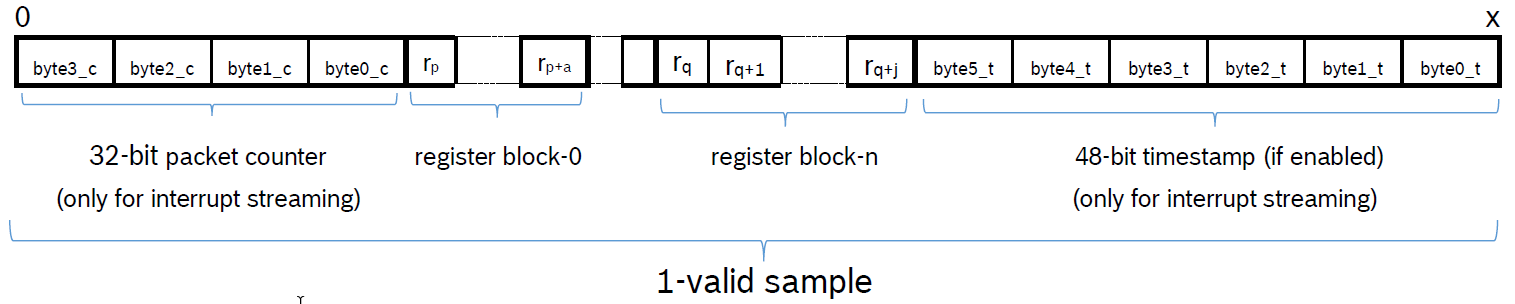
\includegraphics[width=\textwidth]{coinesAPI_images/COINES_streamingSample}
	\caption{Format of streaming packages}
\end{figure}

In the above figure, the following meaning apply to the mentioned abreviations:
\begin{itemize}
	\item r\textsubscript{p}: Value at register address p
	\item a: Size of register block–0
	\item r\textsubscript{p+a}: Value at register address p
\end{itemize}

Similarly is the case for r\textsubscript{q}, j and r\textsubscript{q+j}. See the \texttt{coines\_streaming\_blocks} structure for information regarding register blocks.

The packet counter and the timestamp can be obtained as follows:

\begin{itemize}
	\item[] \texttt{packet\_counter = (byte3\_c << 24) | (byte2\_c << 16) | (byte1\_c << 8) | (byte0\_c)}
	\item[] \texttt{timestamp = (byte5\_t << 40) | (byte4\_t << 32) | (byte3\_t << 24) | (byte2\_t << 16) | (byte1\_t << 8) | (byte0\_t)}
\end{itemize}

The 48-bit timestamp is enabled by using \\ \texttt{coines\_trigger\_timer(COINES\_TIMER\_START,  COINES\_TIMESTAMP\_ENABLE);}

Timestamp in microseconds can be obtained using below formula:
\begin{itemize}
	\item[] $\displaystyle Timestamp\ (\mu s) = \frac{48bit\_timestamp}{30}$
\end{itemize}

\paragraph{coines\_trigger\_timer}
Triggers the timer in firmware and also enables or disables the time stamp feature.

\begin{lstlisting}
int16_t coines_trigger_timer(enum coines_timer_config tmr_cfg,enum coines_time_stamp_config ts_cfg);
\end{lstlisting}

Arguments:
\begin{itemize}
	\item \texttt{tmr\_cfg}: start, stop or reset the timer (\texttt{COINES\_TIMER\_START}, \texttt{COINES\_TIMER\_STOP} or \\ \texttt{COINES\_TIMER\_RESET}) 
	\item \texttt{ts\_cfg}: Enables/disables microcontroller timestamp  (\texttt{COINES\_TIMESTAMP\_ENABLE} or \\ \texttt{COINES\_TIMESTAMP\_DISABLE}) 
\end{itemize}

\subsubsection{coinesAPI calls: Other useful APIs}
\paragraph{coines\_get\_millis}
Returns the number of milliseconds passed since the program started

\begin{lstlisting}
uint32_t coines_get_millis();
\end{lstlisting}

\paragraph{coines\_get\_micro\_sec}
Returns the number of microseconds passed since the program started

\begin{lstlisting}
uint64_t coines_get_micro_sec();
\end{lstlisting}

\paragraph{coines\_attach\_interrupt}
Attaches an interrupt to a Multi-IO pin.Works only on MCU.

\begin{lstlisting}
void coines_attach_interrupt(enum coines_multi_io_pin pin_number,void (*callback)(uint32_t, uint32_t),enum coines_pin_interrupt_mode int_mode);
\end{lstlisting}

Arguments:
\begin{itemize}
	\item \texttt{pin\_number}:  Multi-IO pin
	\item \texttt{callback}: Name of the function to be called on detection of interrupt
	\item \texttt{int\_mode}: Trigger modes - change (\texttt{COINES\_PIN\_INTERRUPT\_CHANGE}), \\
	rising edge (\texttt{COINES\_PIN\_INTERRUPT\_RISING\_EDGE}), \\falling edge (\texttt{COINES\_PIN\_INTERRUPT\_FALLING\_EDGE})
\end{itemize}

\paragraph{coines\_detach\_interrupt}
Detaches interrupt from a Multi-IO pin.Works only on MCU.

\begin{lstlisting}
void coines_detach_interrupt(enum coines_multi_io_pin pin_number);
\end{lstlisting}

Arguments:
\begin{itemize}
	\item \texttt{pin\_number}: Multi-IO pin.
\end{itemize}

\paragraph{coines\_intf\_available}
Return the number of bytes available in the read buffer of the interface.Works only on APP3.x MCU target.

\begin{lstlisting}
uint16_t coines_intf_available(enum coines_comm_intf intf);
\end{lstlisting}

Arguments:
\begin{itemize}
	\item \texttt{intf}: Type of interface (USB, COM, or BLE)
\end{itemize}

\paragraph{coines\_intf\_connected}
Check if the interface is connected.Works only on APP3.x MCU target.

\begin{lstlisting}
bool coines_intf_connected(enum coines_comm_intf intf);
\end{lstlisting}

Arguments:
\begin{itemize}
	\item \texttt{intf}: Type of interface (USB, COM, or BLE)
\end{itemize}

\paragraph{coines\_flush\_intf}
Flush the write buffer.Works only on APP3.x MCU target.

\begin{lstlisting}
void coines_flush_intf(enum coines_comm_intf intf);
\end{lstlisting}

Arguments:
\begin{itemize}
	\item \texttt{intf}: Type of interface (USB, COM, or BLE)
\end{itemize}

\paragraph{coines\_read\_intf}
Read data over the specified interface.Works only on APP3.x MCU target.

\begin{lstlisting}
uint16_t coines_read_intf(enum coines_comm_intf intf, void *buffer, uint16_t len);
\end{lstlisting}

Arguments:
\begin{itemize}
	\item \texttt{intf}: Type of interface (USB, COM, or BLE)
	\item \texttt{buffer}: Pointer to the buffer to store the data
	\item \texttt{len}: Length of the buffer
\end{itemize}

\paragraph{coines\_write\_intf}
Write data over the specified interface.Works only on APP3.x MCU target.

\begin{lstlisting}
uint16_t coines_write_intf(enum coines_comm_intf intf, void *buffer, uint16_t len);
\end{lstlisting}

Arguments:
\begin{itemize}
	\item \texttt{intf}: Type of interface (USB, COM, or BLE)
	\item \texttt{buffer}: Pointer to the buffer storing the data
	\item \texttt{len}: Length of the buffer
\end{itemize}

\paragraph{coines\_get\_version}
Returns pointer to COINES version string

\begin{lstlisting}
char* coines_get_version(void);
\end{lstlisting}

\paragraph{coines\_soft\_reset}
Resets the device. After reset device jumps to the address specified in makefile(APP\_START\_ADDRESS).

\begin{lstlisting}
void coines_soft_reset(void);
\end{lstlisting}

\paragraph{coines\_read\_temp\_data}
This API is used to read the temperature sensor data.

\begin{lstlisting}
int16_t coines_read_temp_data(float *temp_data);
\end{lstlisting}
        
Arguments:
\begin{itemize}
	\item \texttt{temp\_conv\_data}: Buffer to retrieve the sensor data in degree Celsius.
\end{itemize}

\paragraph{coines\_read\_bat\_status}
This API is used to read the battery status.

\begin{lstlisting}
int16_t coines_read_bat_status(uint16_t *bat_status_mv, uint8_t *bat_status_percent);
\end{lstlisting}

Arguments:
\begin{itemize}
	\item \texttt{bat\_status\_mv}: Buffer to retrieve the battery status in millivolt
	\item \texttt{bat\_status\_percent}: Buffer to retrieve the battery status in percentage
\end{itemize}

\paragraph{coines\_ble\_config}
This API is used to configure BLE name and power. It should be called before calling coines\_open\_comm\_intf API.

\begin{lstlisting}
int16_t coines_ble_config(struct coines_ble_config *ble_config);
\end{lstlisting}

Arguments:
\begin{itemize}
	\item \texttt{ble\_config}: structure holding ble name and power details
\end{itemize}

\paragraph{coines\_set\_led}
 This API is used to set led state(on or off).
 
\begin{lstlisting}
int16_t coines_set_led(enum coines_led led,enum coines_led_state led_state);
\end{lstlisting}

Arguments:
\begin{itemize}
	\item \texttt{led}: led to which the state has to be set.
	\item \texttt{led\_state}: state to be set to the given led.
\end{itemize}

\paragraph{coines\_timer\_config}
 This API is used to configure the hardware timer.
 
\begin{lstlisting}
int16_t coines_timer_config(enum coines_timer_instance instance, void* handler);
\end{lstlisting}

Arguments:
\begin{itemize}
	\item \texttt{instance}: timer instance.
	\item \texttt{handler}: callback to be called when timer expires.
\end{itemize}

\paragraph{coines\_timer\_deconfig}
 This API is used to de-configure the hardware timer.
 
\begin{lstlisting}
int16_t coines_timer_deconfig(enum coines_timer_instance instance);
\end{lstlisting}

Arguments:
\begin{itemize}
	\item \texttt{instance}: timer instance.
\end{itemize}

\paragraph{coines\_timer\_start}
 This API is used to start the configured hardware timer.
 
\begin{lstlisting}
int16_t coines_timer_start(enum coines_timer_instance instance, uint32_t timeout);
\end{lstlisting}

Arguments:
\begin{itemize}
	\item \texttt{instance}: timer instance.
	\item \texttt{timeout}: timeout in microseconds.
\end{itemize}

\paragraph{coines\_timer\_stop}
 This API is used to stop the  hardware timer.
 
\begin{lstlisting}
int16_t coines_timer_stop(enum coines_timer_instance instance);
\end{lstlisting}

Arguments:
\begin{itemize}
	\item \texttt{instance}: timer instance.
\end{itemize}

\paragraph{coines\_get\_realtime\_usec}
This API is used to get the current counter(RTC) reference time in usec

\begin{lstlisting}
uint32_t coines_get_realtime_usec(void);
\end{lstlisting}

\paragraph{coines\_delay\_realtime\_usec}
This API is used to introduce delay based on high precision RTC(LFCLK crystal) with the resolution of 30.517 usec.

\begin{lstlisting}
void coines_delay_realtime_usec(uint32_t period);
\end{lstlisting}

Arguments:
\begin{itemize}
	\item \texttt{period}: required delay in microseconds 
\end{itemize}

\paragraph{coines\_attach\_timed\_interrupt}
Attaches a timed interrupt to a Multi-IO pin.

\begin{lstlisting}
int16_t coines_attach_timed_interrupt(enum coines_multi_io_pin pin_number, void (*timed_interrupt_cb)(uint64_t,uint32_t,uint32_t), enum coines_pin_interrupt_mode int_mode);
\end{lstlisting}

Arguments:
\begin{itemize}
	\item \texttt{pin\_number}: Multi-IO pin.
	\item \texttt{timed\_interrupt\_cb}: Name of the function to be called on detection of interrupt.
	\item \texttt{int\_mode}: Trigger modes - change,rising edge,falling edge.
\end{itemize}

\paragraph{coines\_detach\_timed\_interrupt}
Detaches a timed interrupt from a Multi-IO pin.

\begin{lstlisting}
int16_t coines_detach_timed_interrupt(enum coines_multi_io_pin pin_number);
\end{lstlisting}

Arguments:
\begin{itemize}
	\item \texttt{pin\_number}: Multi-IO pin.
\end{itemize}

\paragraph{coines\_echo\_test}
This API is used to test the communication.

\begin{lstlisting}
int16_t coines_echo_test(uint8_t *data, uint16_t length);
\end{lstlisting}

Arguments:
\begin{itemize}
	\item \texttt{data}: Data to be sent for testing.
	\item \texttt{length}: Length of the data.
\end{itemize}

\paragraph{coines\_shuttle\_eeprom\_write}
This API is used to write the content into shuttle eeprom.

\begin{lstlisting}
int16_t coines_shuttle_eeprom_write(uint16_t start_addr, uint8_t *buffer, uint16_t length);
\end{lstlisting}

Arguments:
\begin{itemize}
	\item \texttt{start\_addr}: EEPROM write address.
	\item \texttt{buffer}: Pointer to the buffer.
	\item \texttt{length}: Length of the buffer.
\end{itemize}

\paragraph{coines\_shuttle\_eeprom\_read}
This API is used to read the content from shuttle eeprom.

\begin{lstlisting}
int16_t coines_shuttle_eeprom_read(uint16_t start_addr, uint8_t *buffer, uint16_t length);
\end{lstlisting}

Arguments:
\begin{itemize}
	\item \texttt{start\_addr}: EEPROM read address.
	\item \texttt{buffer}: Pointer to the buffer.
	\item \texttt{length}: Length of the buffer.
\end{itemize}

\paragraph{coines\_yield}
This API can be defined to perform a task when yielded from an ongoing blocking call.

\begin{lstlisting}
void coines_yield(void);
\end{lstlisting}

\paragraph{coines\_execute\_critical\_region}
This API is used to execute the function inside critical region.

\begin{lstlisting}
void coines_execute_critical_region(coines_critical_callback callback);
\end{lstlisting}

Arguments:
\begin{itemize}
	\item \texttt{callback}: function to execute.
\end{itemize}

\paragraph{coines\_scan\_ble\_devices}\label{coinesScanBleDevices}
This API is used to connect to BLE Adapter and return list of BLE peripherals found during BLE scan.

\begin{lstlisting}
	int16_t coines_scan_ble_devices(struct ble_peripheral_info *ble_info, uint8_t *peripheral_count, size_t scan_timeout_ms)
\end{lstlisting}

Arguments:
\begin{itemize}
	\item \texttt{ble\_info}: array of struct containing found BLE peripheral information
	\item \texttt{peripheral\_count}: number of BLE peripherals found
	\item \texttt{scan\_timeout\_ms}: timeout for BLE scan
\end{itemize}

\newpage


\newpage
\subsection{COINES Python functions}

As coinespy is only a wrapper on top of coinesAPI, the following API documentation is limited to the wrapper only. Details about meaning of variables and functionality can be found in the corresponding coinesAPI documentation in the chapter above.
\vspace{12pt}
The following function calls are defined within the class \texttt{CoinesBoard}. Thus in order to access the functions, the user has to create an object of that class first.

\begin{lstlisting}[language=python]
	import coinespy as cpy
	coinesboard = cpy.CoinesBoard()
\end{lstlisting}

\subsubsection{coinespy API calls: Interface and board information}

\paragraph{open\_comm\_interface}
Sets the communication interface between board and PC to USB, Serial or BLE.

\begin{lstlisting}[language=python]
coinesboard.open_comm_interface(interface=CommInterface.USB, serial_com_config: SerialComConfig = None,
ble_com_config: BleComConfig = None) -> ErrorCodes
\end{lstlisting}

For the definition of \texttt{CommInterface}, refer to \ref{CommInterface}.

\paragraph{close\_comm\_interface}
Disposes the resources used by the USB/serial/BLE communication.

\begin{lstlisting}[language=python]
coinesboard.close_comm_interface(arg=None) -> ErrorCodes
\end{lstlisting}

\paragraph{get\_board\_info}
Obtains board specific information.

\begin{lstlisting}[language=python]
BoardInfo = coinesboard.get_board_info()

# Return:
BoardInfo.HardwareId    # Hardware ID
BoardInfo.SoftwareId    # Firmware version information
BoardInfo.Board         # Board type
BoardInfo.ShuttleID     # ID of shuttle, in case a shuttle is detected
\end{lstlisting}

\paragraph{scan\_ble\_devices}
This API is used to connect to BLE Adapter and return list of BLE peripherals found during BLE scan.

\begin{lstlisting}
ble_info, peripheral_count  = coinesboard.scan_ble_devices(scan_timeout_ms=0) -> Tuple[list, int]
\end{lstlisting}

For the definition of parameters, refer to \ref{coinesScanBleDevices}.

\paragraph{echo\_test}
This API is used to test the communication.

\begin{lstlisting}
coinesboard.echo_test(data: List[int]) -> ErrorCodes
\end{lstlisting}

Arguments:
\begin{itemize}
	\item \texttt{data}: Data to be sent for testing.
\end{itemize}

\subsubsection{coinespy API calls: GPIO oriented calls}

\paragraph{set\_pin\_config}
Configures the state, level and direction of a GPIO pin

\begin{lstlisting}[language=python]
coinesboard.set_pin_config(pin_number: MultiIOPin, direction: PinDirection, output_state: PinValue) -> ErrorCodes
\end{lstlisting}

For the definition of \texttt{MultiIOPin}, refer to \ref{MultiIOPin}. For the definition of \texttt{PinDirection}, refer to \ref{PinDirection}.
For \texttt{PinValue}, refer to \ref{PinValue}.

\paragraph{get\_pin\_config}
Obtains information regarding the Pin's state, level and direction.

\begin{lstlisting}[language=python]
PinConfigInfo = coinesboard.get_pin_config(pin_number: MultiIOPin)

# Return:
PinConfigInfo.direction         # 0: INPUT, 1: OUTPUT
PinConfigInfo.switch_state       # 0: OFF, 1: ON
PinConfigInfo.level             # 1: HIGH, 0: LOW
\end{lstlisting}

\paragraph{set\_shuttleboard\_vdd\_vddio\_config}

Set the VDD and VDDIO voltage level.

\begin{lstlisting}
coinesboard.set_shuttleboard_vdd_vddio_config(vdd_val: float = None, vddio_val: float = None) -> ErrorCodes

# Example: coinesboard.set_shuttleboard_vdd_vddio_config(3.3, 3.3)
\end{lstlisting}

\paragraph{set\_vdd}

Set the VDD voltage level.

\begin{lstlisting}
coinesboard.set_vdd(vdd_val: float = None) -> ErrorCodes

# Example: coinesboard.set_vdd(3.3)
\end{lstlisting}

\paragraph{set\_vddio}

Set the VDDIO voltage level.

\begin{lstlisting}
coinesboard.set_vddio(vdd_val: float = None) -> ErrorCodes

# Example: coinesboard.set_vddio(3.3)
\end{lstlisting}

\subsubsection{coinespy API calls: Sensor communication}

For the definition of \texttt{SPIBus}, refer to \ref{SPIBus}. For the definition of \texttt{I2CBus}, refer to \ref{I2CBus}.

\paragraph{config\_i2c\_bus}
Configures the I\textsuperscript{2}C bus.

\begin{lstlisting}
coinesboard.config_i2c_bus(bus: I2CBus, i2c_address: int, i2c_mode: I2CMode) -> ErrorCodes
\end{lstlisting}

For the definition of \texttt{I2CMode}, refer to \ref{I2CMode}.

\paragraph{config\_spi\_bus}
Configures the SPI bus of the board.
\begin{lstlisting}
coinesboard.config_spi_bus(bus: SPIBus, cs_pin: MultiIOPin, spi_speed=SPISpeed, spi_mode=SPIMode) -> ErrorCodes
\end{lstlisting}

For the definition of \texttt{MultiIOPin}, refer to \ref{MultiIOPin}. For the definition of \texttt{SPISpeed}, refer to \ref{SPISpeed}. For the definition of \texttt{SPIMode}, refer to \ref{SPIMode}.

\paragraph{deconfig\_i2c\_bus}
This API is used to de-configure the I\textsuperscript{2}C bus

\begin{lstlisting}
coinesboard.deconfig_i2c_bus(bus: I2CBus) -> ErrorCodes
\end{lstlisting}

\paragraph{deconfig\_spi\_bus}
This API is used to de-configure the SPI bus

\begin{lstlisting}
coinesboard.deconfig_spi_bus(bus: SPIBus) -> ErrorCodes
\end{lstlisting}

\paragraph{write\_i2c}
Writes 8-bit register data to the I\textsuperscript{2}C

\begin{lstlisting}
coinesboard.write_i2c(bus: I2CBus, register_address: int, register_value: int, sensor_interface_detail: int = None) -> ErrorCodes
\end{lstlisting}

For the definition of parameters, refer to \ref{CoinesWriteI2c}.

\paragraph{read\_i2c}
Reads 8-bit register data from the I\textsuperscript{2}C

\begin{lstlisting}
register_data = coinesboard.read_i2c(bus: I2CBus, register_address: int, number_of_reads=1, sensor_interface_detail: int = None)
\end{lstlisting}

For the definition of parameters, refer to \ref{CoinesReadI2c}.

\paragraph{write\_spi}
Writes 8-bit register data to the SPI device

\begin{lstlisting}
coinesboard.write_spi(bus: SPIBus, register_address: int, register_value: int, sensor_interface_detail: int = None) -> ErrorCodes
\end{lstlisting}


For the definition of parameters, refer to \ref{CoinesWriteSpi}.

\paragraph{read\_spi}
Reads 8-bit register data from the SPI device.

\begin{lstlisting}
register_data = coinesboard.read_spi(bus: SPIBus, register_address: int, number_of_reads=1, sensor_interface_detail: int = None)
\end{lstlisting}

For the definition of parameters, refer to \ref{CoinesReadSpi}.

\paragraph{delay\_milli\_sec}
Introduces delay in millisecond.

\begin{lstlisting}
coinesboard.delay_milli_sec(time_in_milli_sec=100)
\end{lstlisting}

\paragraph{delay\_micro\_sec}
Introduces delay in microsecond.

\begin{lstlisting}
coinesboard.delay_micro_sec(time_in_micro_sec=1)
\end{lstlisting}

\subsubsection{coinespy API calls: Streaming feature}

\paragraph{config\_streaming}

Sets the configuration for streaming sensor data.

\begin{lstlisting}[language=python]
coinesboard.config_streaming(sensor_id: int,
	stream_config: StreamingConfig, data_blocks: StreamingBlocks) -> ErrorCodes
\end{lstlisting}

Arguments:
\begin{itemize}
	\item \texttt{sensor\_id}: An integer number that can be used as identifier/index to the sensor data that will be streamed for this setting

	\item \texttt{stream\_config}: Contains information regarding interface settings and streaming configuration.
	\item  \texttt{data\_blocks}: Contains information regarding numbers of blocks to read, register address and size for each block.
\end{itemize}
Note:\newline
The below parameters should always be set:
\begin{itemize}
	\item \texttt{data\_blocks.NoOfBlocks}: number of blocks to stream (must at least be one)
	\item For each block b:
	      \begin{itemize}
		      \item \texttt{data\_blocks.RegStartAddr[b]}: start address of the block in the register map
		      \item \texttt{data\_blocks.NoOfDataBytes[b]}: number of bytes to read, starting from the start address
	      \end{itemize}
\end{itemize}
\vspace{12pt}
For reading data from I\textsuperscript{2}C bus,then set the below parameters:
\begin{itemize}
	\item \texttt{stream\_config.Intf = cpy.SensorInterface.I2C.value}
	\item \texttt{stream\_config.I2CBus}: I\textsuperscript{2}C bus (in case of APP2.0 and APP3.x, this is always\\
	      \texttt{cpy.I2CBus.BUS\_I2C\_0.value})
	\item \texttt{stream\_config.DevAddr}: I\textsuperscript{2}C address of the sensor
\end{itemize}
\vspace{12pt}
For reading data from SPI bus, then set the below parameters:
\begin{itemize}
	\item \texttt{stream\_config.Intf = cpy.SensorInterface.SPI.value;}
	\item \texttt{stream\_config.SPIBus}: SPI bus (in case of APP2.0 and APP3.x, this is always\\
	      \texttt{cpy.SPIBus.BUS\_SPI\_0.value})
	\item \texttt{stream\_config.CSPin}: CS pin of the sensor, information can be obtained from the shuttle board documentation for the sensor.
	\item \texttt{stream\_config.SPIType}: 0 : 8-bit SPI; 1 : 16-bit SPI
\end{itemize}
\vspace{12pt}
When polling mode is requested, set the below parameters:
\begin{itemize}
	\item \texttt{stream\_config.SamplingUnits}: either milliseconds or microseconds. Refer to \ref{SamplingUnits}.
	\item \texttt{stream\_config.SamplingTime}: sampling period in the unit as defined in \\ \texttt{stream\_config.SamplingUnits}
\end{itemize}
\vspace{12pt}
When interrupt mode is requested, set the below parameters:
\begin{itemize}
	\item \texttt{stream\_config.IntPin}: pin of the interrupt which shall trigger the sensor read-out. If the interrupt output of the sensor is used, the required information about the pin number can be obtained from the shuttle board documentation for the sensor.
	\item \texttt{stream\_config.IntTimeStamp}:  it can be configured if the sensor data is tagged with a timestamp - 1 or not - 0.
	\item \texttt{stream\_config.HwPinState}: State of the hardware pin connected to the interrupt line - 0/1 : Low/high
\end{itemize}
\vspace{12pt}
Below parameters are common for both streaming types:
\begin{itemize}
	\item \texttt{stream\_config.IntlineCount}: Number of interrupt lines to be used for monitoring interrupts.
	\item \texttt{stream\_config.IntlineInfo}: List of pin numbers that correspond to interrupt lines being used for interrupt monitoring.
	\item \texttt{stream\_config.ClearOnWrite}: 0/1 : Disable/enable "clear on write" feature
\end{itemize}
\vspace{12pt}
The below parameters should be set only when stream\_config.ClearOnWrite = 1:
\begin{itemize}
	\item \texttt{stream\_config.ClearOnWriteConfig.StartAddress}: Address of the sensor register at which the process of clearOnWrite should initiate.
	\item \texttt{stream\_config.ClearOnWriteConfig.DummyByte}: Number of padding bytes that must be added before clearing the bytes starting from the designated address.
	\item \texttt{stream\_config.ClearOnWriteConfig.NumBytesToClear}: Number of bytes that need to be cleared.
\end{itemize}
\vspace{12pt}
Below is the Python code snippet for interrupt streaming
\begin{lstlisting}[language=Python]
# Store streaming settings in local variables
accel_stream_settings = dict(
	I2C_ADDR_PRIMARY=0x18,
	NO_OF_BLOCKS = 2,
	REG_X_LSB= [0x12, 0x00],
	NO_OF_DATA_BYTES= [6, 1],
	CHANNEL_ID=1,
	CS_PIN=cpy.MultiIOPin.SHUTTLE_PIN_8.value,
	INT_PIN=cpy.MultiIOPin.SHUTTLE_PIN_21.value,
	INT_TIME_STAMP=1,
)
gyro_stream_settings = dict(
	I2C_ADDR_PRIMARY=0x68,
	NO_OF_BLOCKS = 2,
	REG_X_LSB= [0x02,0x00],
	NO_OF_DATA_BYTES = [6, 1],
	CHANNEL_ID=2,
	CS_PIN=cpy.MultiIOPin.SHUTTLE_PIN_14.value,
	INT_PIN=cpy.MultiIOPin.SHUTTLE_PIN_22.value,
	INT_TIME_STAMP=1,
)


# set the config_streaming parameters
stream_config = cpy.StreamingConfig()
data_blocks = cpy.StreamingBlocks()
if self.interface == cpy.SensorInterface.I2C:
	stream_config.Intf = cpy.SensorInterface.I2C.value
	stream_config.I2CBus = cpy.I2CBus.BUS_I2C_0.value
	stream_config.DevAddr = sensor["I2C_ADDR_PRIMARY"]

elif self.interface == cpy.SensorInterface.SPI:
	stream_config.Intf = cpy.SensorInterface.SPI.value
	stream_config.SPIBus = cpy.SPIBus.BUS_SPI_0.value
	stream_config.CSPin = sensor["CS_PIN"]

if sensor_type == bmi08x.SensorType.ACCEL and self.interface == cpy.SensorInterface.SPI:
	# extra dummy byte for SPI
	dummy_byte_offset = 1
else:
	dummy_byte_offset = 0

data_blocks.NoOfBlocks = sensor["NO_OF_BLOCKS"]
for i in range(0, data_blocks.NoOfBlocks):
	data_blocks.RegStartAddr[i] = sensor["REG_X_LSB"][i]
	data_blocks.NoOfDataBytes[i] = sensor["NO_OF_DATA_BYTES"][i] + dummy_byte_offset

stream_config.IntTimeStamp = sensor["INT_TIME_STAMP"]
stream_config.IntPin = sensor["INT_PIN"]

# call config_streaming API for each sensor to configure the streaming settings
ret = coinesboard.config_streaming(
	accel_sensor_id, self.accel_stream_config, self.accel_data_blocks)
ret = coinesboard.config_streaming(
	gyro_sensor_id, self.accel_stream_config, self.accel_data_blocks)

\end{lstlisting}



\paragraph{start\_stop\_streaming}

Starts or stops sensor data streaming.

\begin{lstlisting}[language=python]
coinesboard.start_stop_streaming(stream_mode: StreamingMode, start_stop: StreamingState) -> ErrorCodes
\end{lstlisting}

For the definition of \texttt{StreamingMode}, refer to \ref{StreamingMode}. For the definition of \texttt{StreamingState}, refer to \ref{StreamingState}.

\paragraph{read\_stream\_sensor\_data}

Reads the data streamed from the sensor.

\begin{lstlisting}[language=python]
coinesboard.read_stream_sensor_data(sensor_id: int, number_of_samples: int,
	buffer_size=STREAM_RSP_BUF_SIZE) -> Tuple[ErrorCodes, list, int]
\end{lstlisting}

Return:\\
Tuple of ErrorCodes, data and valid\_samples\_count\newline
For the detailed definition of parameters, refer to \ref{coinesReadStreamSensorData}.

\subsubsection{coinespy API calls: Other useful APIs}

\paragraph{flush\_interface}
Flush the write buffer.

\begin{lstlisting}
coinesboard.flush_interface()
\end{lstlisting}

\paragraph{soft\_reset}
Resets the device.

\begin{lstlisting}
coinesboard.soft_reset()
\end{lstlisting}

\subsubsection{Definition of constants}

\paragraph{PinDirection}\label{PinDirection}

Pin mode definitions

\begin{lstlisting}
class PinDirection:
    INPUT = 0  # COINES_PIN_DIRECTION_IN = 0
    OUTPUT = 1
\end{lstlisting}

\paragraph{PinValue}\label{PinValue}

Pin level definitions

\begin{lstlisting}
class PinValue:
    LOW = 0  # COINES_PIN_VALUE_LOW = 0
    HIGH = 1
\end{lstlisting}

\paragraph{CommInterface}\label{CommInterface}

Definition of Communication interface

\begin{lstlisting}
class CommInterface:
    USB = 0
    SERIAL = 1
    BLE = 2
\end{lstlisting}

\paragraph{I2CMode}\label{I2CMode}

Definition of the speed of I2C bus.

\begin{lstlisting}
class I2CMode:
	STANDARD_MODE = 0 # Standard mode - 100kHz
	FAST_MODE = 1 # Fast mode - 400kHz
	SPEED_3_4_MHZ = 2 # High Speed mode - 3.4 MHz
	SPEED_1_7_MHZ = 3 # High Speed mode 2 - 1.7 MHz
\end{lstlisting}

\paragraph{SPISpeed}\label{SPISpeed}

Definition of the speed of SPI bus.

\begin{lstlisting}
class SPISpeed:
	SPI_10_MHZ = 6
	SPI_7_5_MHZ = 8
	SPI_6_MHZ = 10
	SPI_5_MHZ = 12
	SPI_3_75_MHZ = 16
	SPI_3_MHZ = 20
	SPI_2_5_MHZ = 24
	SPI_2_MHZ = 30
	SPI_1_5_MHZ = 40
	SPI_1_25_MHZ = 48
	SPI_1_2_MHZ = 50
	SPI_1_MHZ = 60
	SPI_750_KHZ = 80
	SPI_600_KHZ = 100
	SPI_500_KHZ = 120
	SPI_400_KHZ = 150
	SPI_300_KHZ = 200
	SPI_250_KHZ = 240
\end{lstlisting}

\paragraph{SPITransferBits}\label{SPITransferBits}

Definition of the SPI bits.

\begin{lstlisting}
class SPITransferBits:
	SPI8BIT = 8 # 8 bit register read/write
	SPI16BIT = 16 # 16 bit register read/write
\end{lstlisting}

\paragraph{SPIMode}\label{SPIMode}

Definition of the SPI mode.

\begin{lstlisting}
class SPIMode:
	MODE0 = 0x00 # SPI Mode 0: CPOL=0; CPHA=0
	MODE1 = 0x01 # SPI Mode 1: CPOL=0; CPHA=1
	MODE2 = 0x02 # SPI Mode 2: CPOL=1; CPHA=0
	MODE3 = 0x03 # SPI Mode 3: CPOL=1; CPHA=1
\end{lstlisting}

\paragraph{MultiIOPin}\label{MultiIOPin}

Definition of the shuttle board pin(s)

\begin{lstlisting}
class MultiIOPin(Enum):
	SHUTTLE_PIN_7 = 0x09 # CS pin
	SHUTTLE_PIN_8 = 0x05 # Multi-IO 5
	SHUTTLE_PIN_9 = 0x00 # Multi-IO 0
	SHUTTLE_PIN_14 = 0x01 # Multi-IO 1
	SHUTTLE_PIN_15 = 0x02 # Multi-IO 2
	SHUTTLE_PIN_16 = 0x03 # Multi-IO 3
	SHUTTLE_PIN_19 = 0x08 # Multi-IO 8
	SHUTTLE_PIN_20 = 0x06 # Multi-IO 6
	SHUTTLE_PIN_21 = 0x07 # Multi-IO 7
	SHUTTLE_PIN_22 = 0x04 # Multi-IO 4
	SHUTTLE_PIN_SDO = 0x1F

	# APP3.x pins
	MINI_SHUTTLE_PIN_1_4 = 0x10  # GPIO0
	MINI_SHUTTLE_PIN_1_5 = 0x11  # GPIO1
	MINI_SHUTTLE_PIN_1_6 = 0x12  # GPIO2/INT1
	MINI_SHUTTLE_PIN_1_7 = 0x13  # GPIO3/INT2
	MINI_SHUTTLE_PIN_2_5 = 0x14  # GPIO4
	MINI_SHUTTLE_PIN_2_6 = 0x15  # GPIO5
	MINI_SHUTTLE_PIN_2_1 = 0x16  # CS
	MINI_SHUTTLE_PIN_2_3 = 0x17  # SDO
	MINI_SHUTTLE_PIN_2_7 = 0x1D  # GPIO6
	MINI_SHUTTLE_PIN_2_8 = 0x1E  # GPIO7
\end{lstlisting}

\paragraph{SensorInterface}\label{SensorInterface}

To define Sensor interface.

\begin{lstlisting}
class SensorInterface(Enum):
	SPI = 0
	I2C = 1
\end{lstlisting}

\paragraph{I2CBus}\label{I2CBus}

Used to define the I2C type.

\begin{lstlisting}
	class I2CBus(Enum):
	BUS_I2C_0 = 0
	BUS_I2C_1 = 1
	BUS_I2C_MAX = 2
\end{lstlisting}

\paragraph{SPIBus}\label{SPIBus}

Used to define the SPI type.

\begin{lstlisting}
	class SPIBus(Enum):
	BUS_SPI_0 = 0
	BUS_SPI_1 = 1
	BUS_SPI_MAX = 2
\end{lstlisting}

\paragraph{PinInterruptMode}\label{PinInterruptMode}

Defines Pin interrupt modes.

\begin{lstlisting}
class PinInterruptMode(Enum):
	# Trigger interrupt on pin state change
	PIN_INTERRUPT_CHANGE = 0
	# Trigger interrupt when pin changes from low to high
	PIN_INTERRUPT_RISING_EDGE = 1
	# Trigger interrupt when pin changes from high to low
	PIN_INTERRUPT_FALLING_EDGE = 2
	PIN_INTERRUPT_MODE_MAXIMUM = 4
\end{lstlisting}

\paragraph{StreamingMode}\label{StreamingMode}

Streaming mode definitions

\begin{lstlisting}
class StreamingMode:
    STREAMING_MODE_POLLING = 0    # Polling mode streaming
    STREAMING_MODE_INTERRUPT = 1  # Interrupt mode streaming
\end{lstlisting}

\paragraph{StreamingState}\label{StreamingState}

Streaming state definitions

\begin{lstlisting}
class StreamingState:
	STREAMING_START = 1
	STREAMING_STOP = 0
\end{lstlisting}

\paragraph{SamplingUnits}\label{SamplingUnits}

Sampling Unit definitions

\begin{lstlisting}
class SamplingUnits:
    SAMPLING_TIME_IN_MICRO_SEC = 0x01  # sampling unit in micro second
    SAMPLING_TIME_IN_MILLI_SEC = 0x02  # sampling unit in milli second
\end{lstlisting}



\newpage

\end{document}